\documentclass[./main.tex]{subfiles}

\begin{document}
\section{Simulation results} \label{sec:simulations}
In the following section we show the results of applying the discrete super learner to a simulated dataset. Our dataset consists of a binary outcome, $Y$, which depends on two covariates $X_1$ and $X_2$. Our setup is as follows
\begin{align*}
    X_1 &\sim \operatorname{Unif}(0.5, 15),\\
    X_2 \mid X_1 = x_1 &\sim \mathcal{N}(3.5-0.03x_1, 1),\\
    Y \mid X_1 = x_1, X_2 = x_2 &\sim \operatorname{Ber}(\theta_0(x_1, x_2)),
\end{align*}
for $\theta_0(x_1, x_2) = \expit({-3.5 - 0.3x_1 + 0.85x_2 + 0.35x_1x_2})$ which is the data-generating regression function. It is in fact possible to visualize the regression function explicitly as a 2-dimensional heat map in the covariates. In figure \ref{fig:trueplot} we have applied the true regression across the grid of $ (x_1, x_2) $ covariate pairs in $ (0, 15) \times (0,7) $ where the spacing is $ 0.5 $ horizontally and vertically between each pair. The probabilities are colored from $ 0 $ to $ 1 $ in the plot. 
\begin{figure}[H]
    \centering
    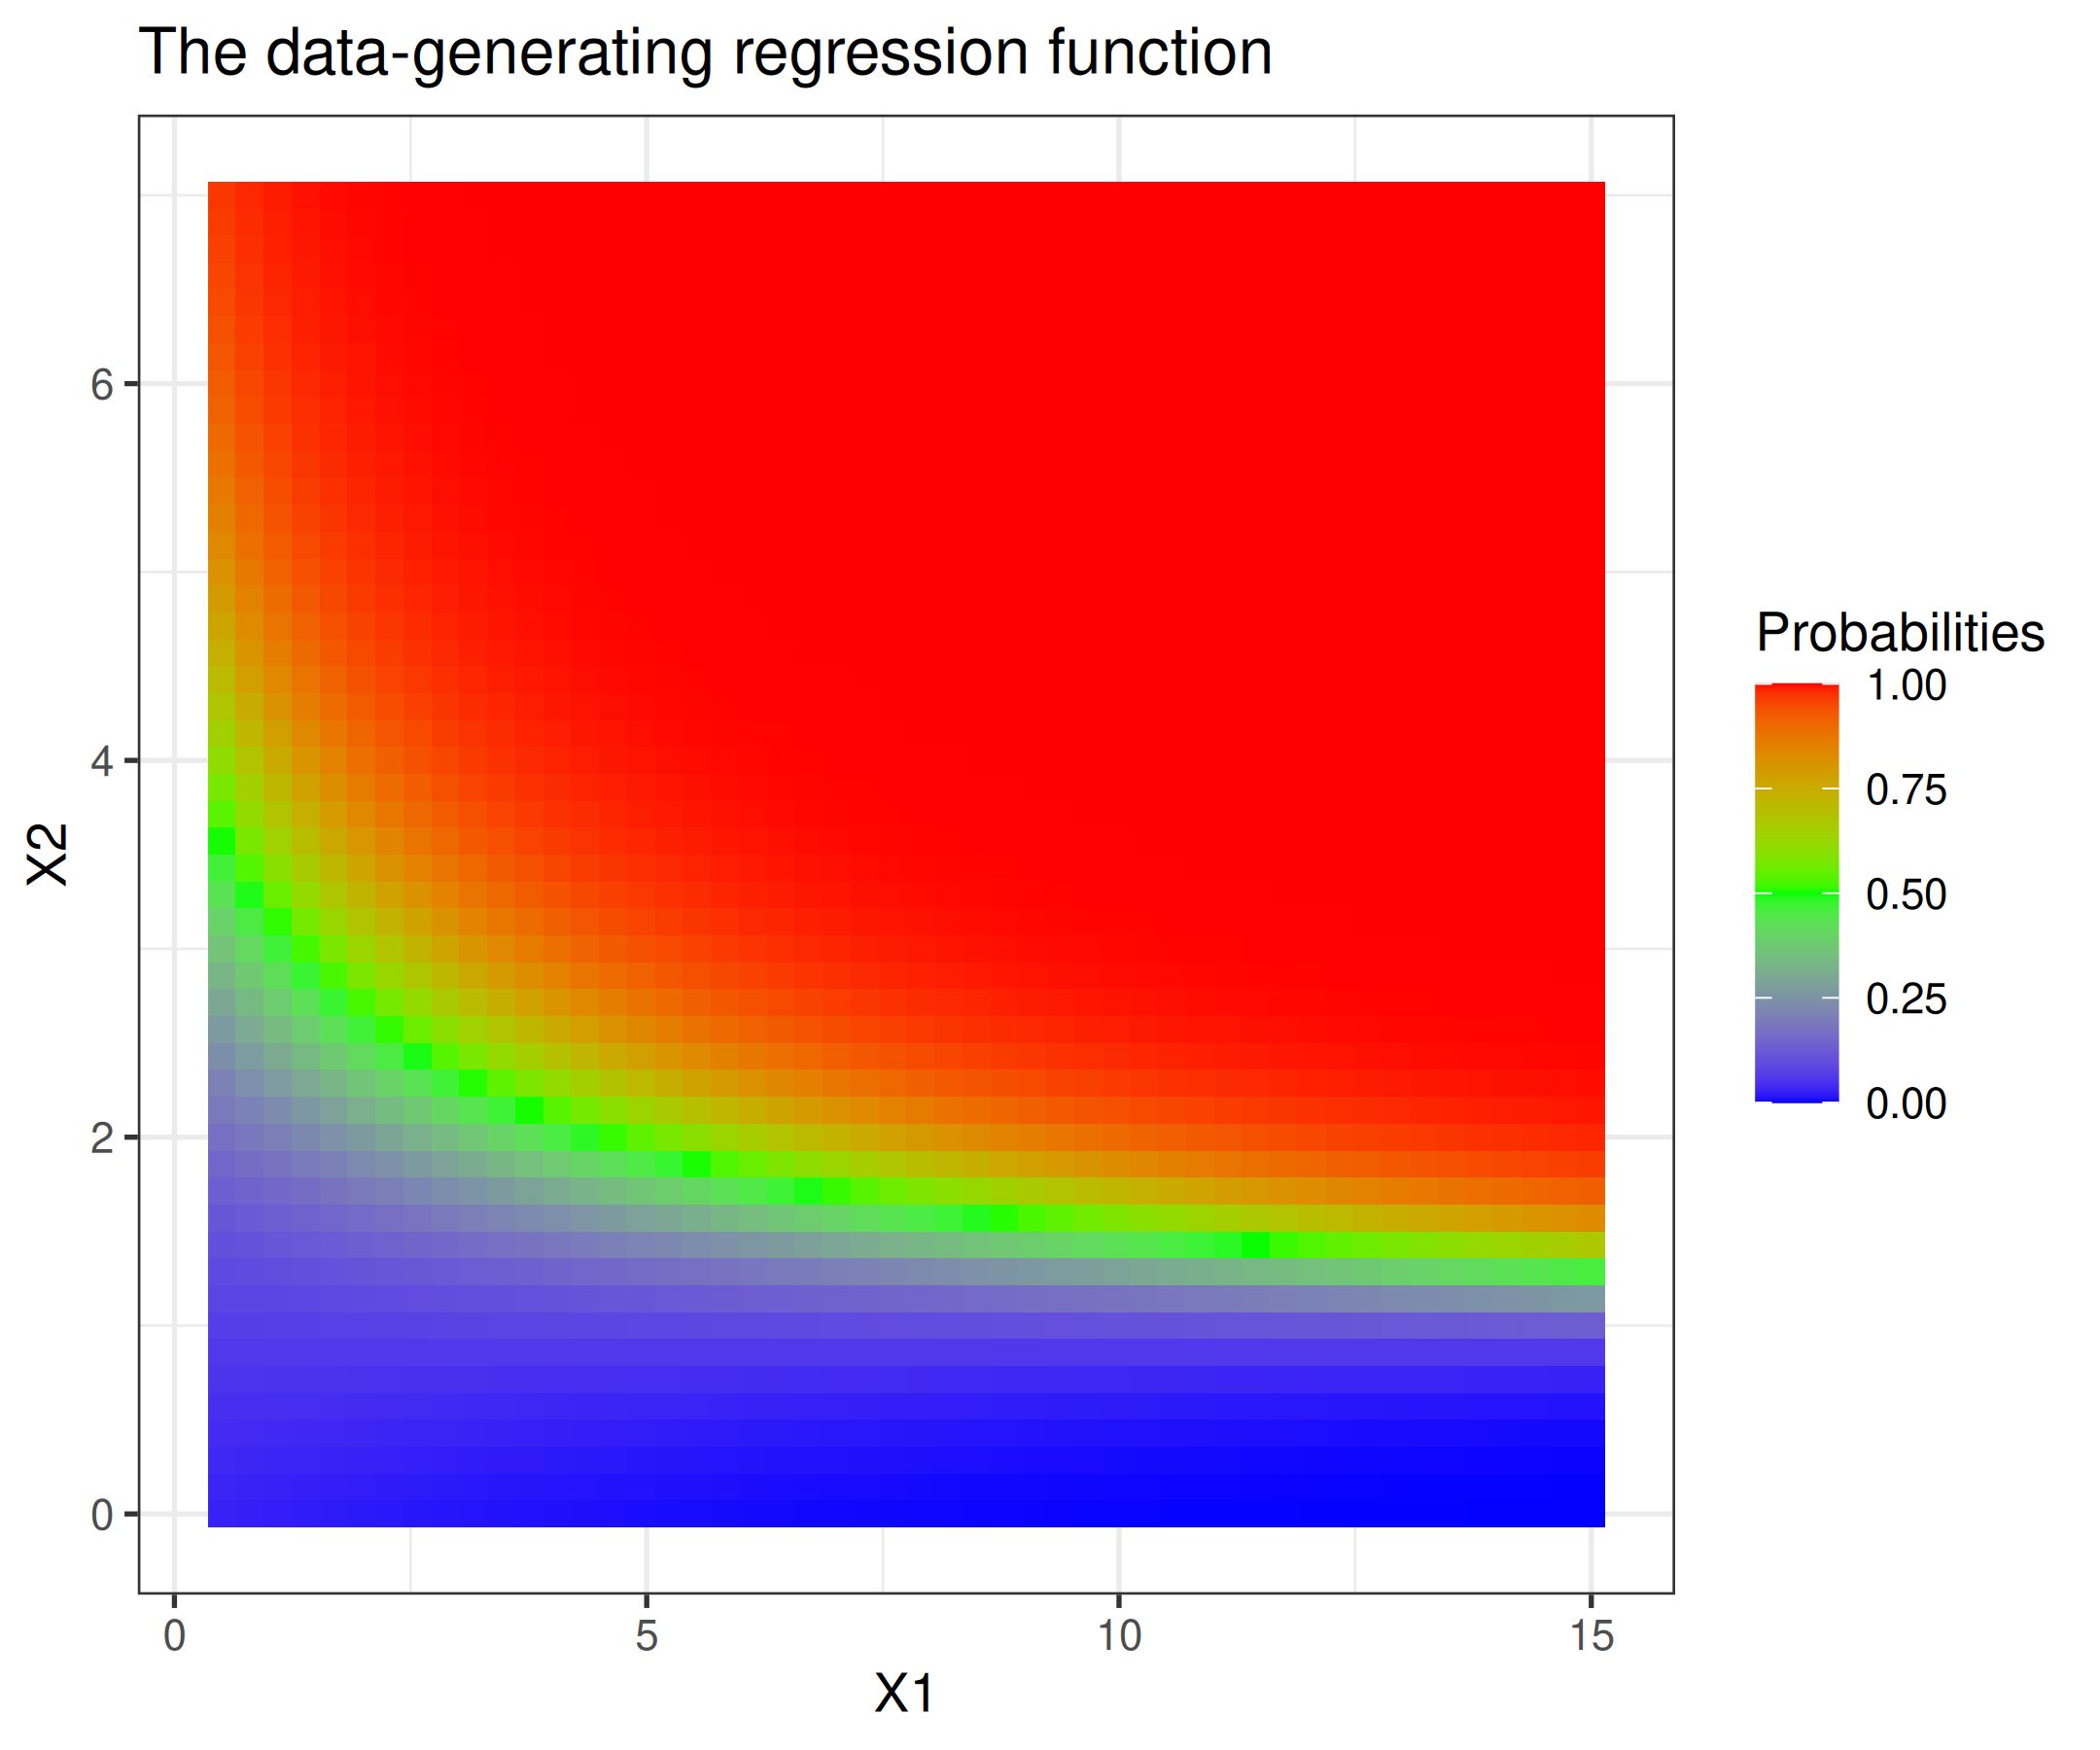
\includegraphics[width=0.8\textwidth]{figures/trueplot.png}
    \caption{The data-generating regression plotted as a heat map}
    \label{fig:trueplot}
\end{figure}
The regression is captured by the logistic regression model with interaction terms. We will use the following library of learning algorithms as an illustrative example:
\begin{enumerate}
    \item Intercept only logistic regression: $E[Y \mid X_1, X_2] = \expit(\beta_0)$
    \item Logistic regression with main effects: $E[Y \mid X_1, X_2] = \expit(\beta_0 + \beta_1 X_1 + \beta_2 X_2)$
    \item XGBoost with hyperparameters: \texttt{max\_depth=3, eta=0.3,\\ n\_rounds=100, objective='binary:logistic', booster='dart', nthread=5}
\end{enumerate}
We can also visualize the predictions of the learning algorithms in the library in the same way as we have done for the data-generating regression. In figure \ref{fig:predictpar} we visualize the predictions of the main effects logistic regression and XGBoost fitted using 1000 observations sampled from the distribution. 
\begin{figure}
    \centering
    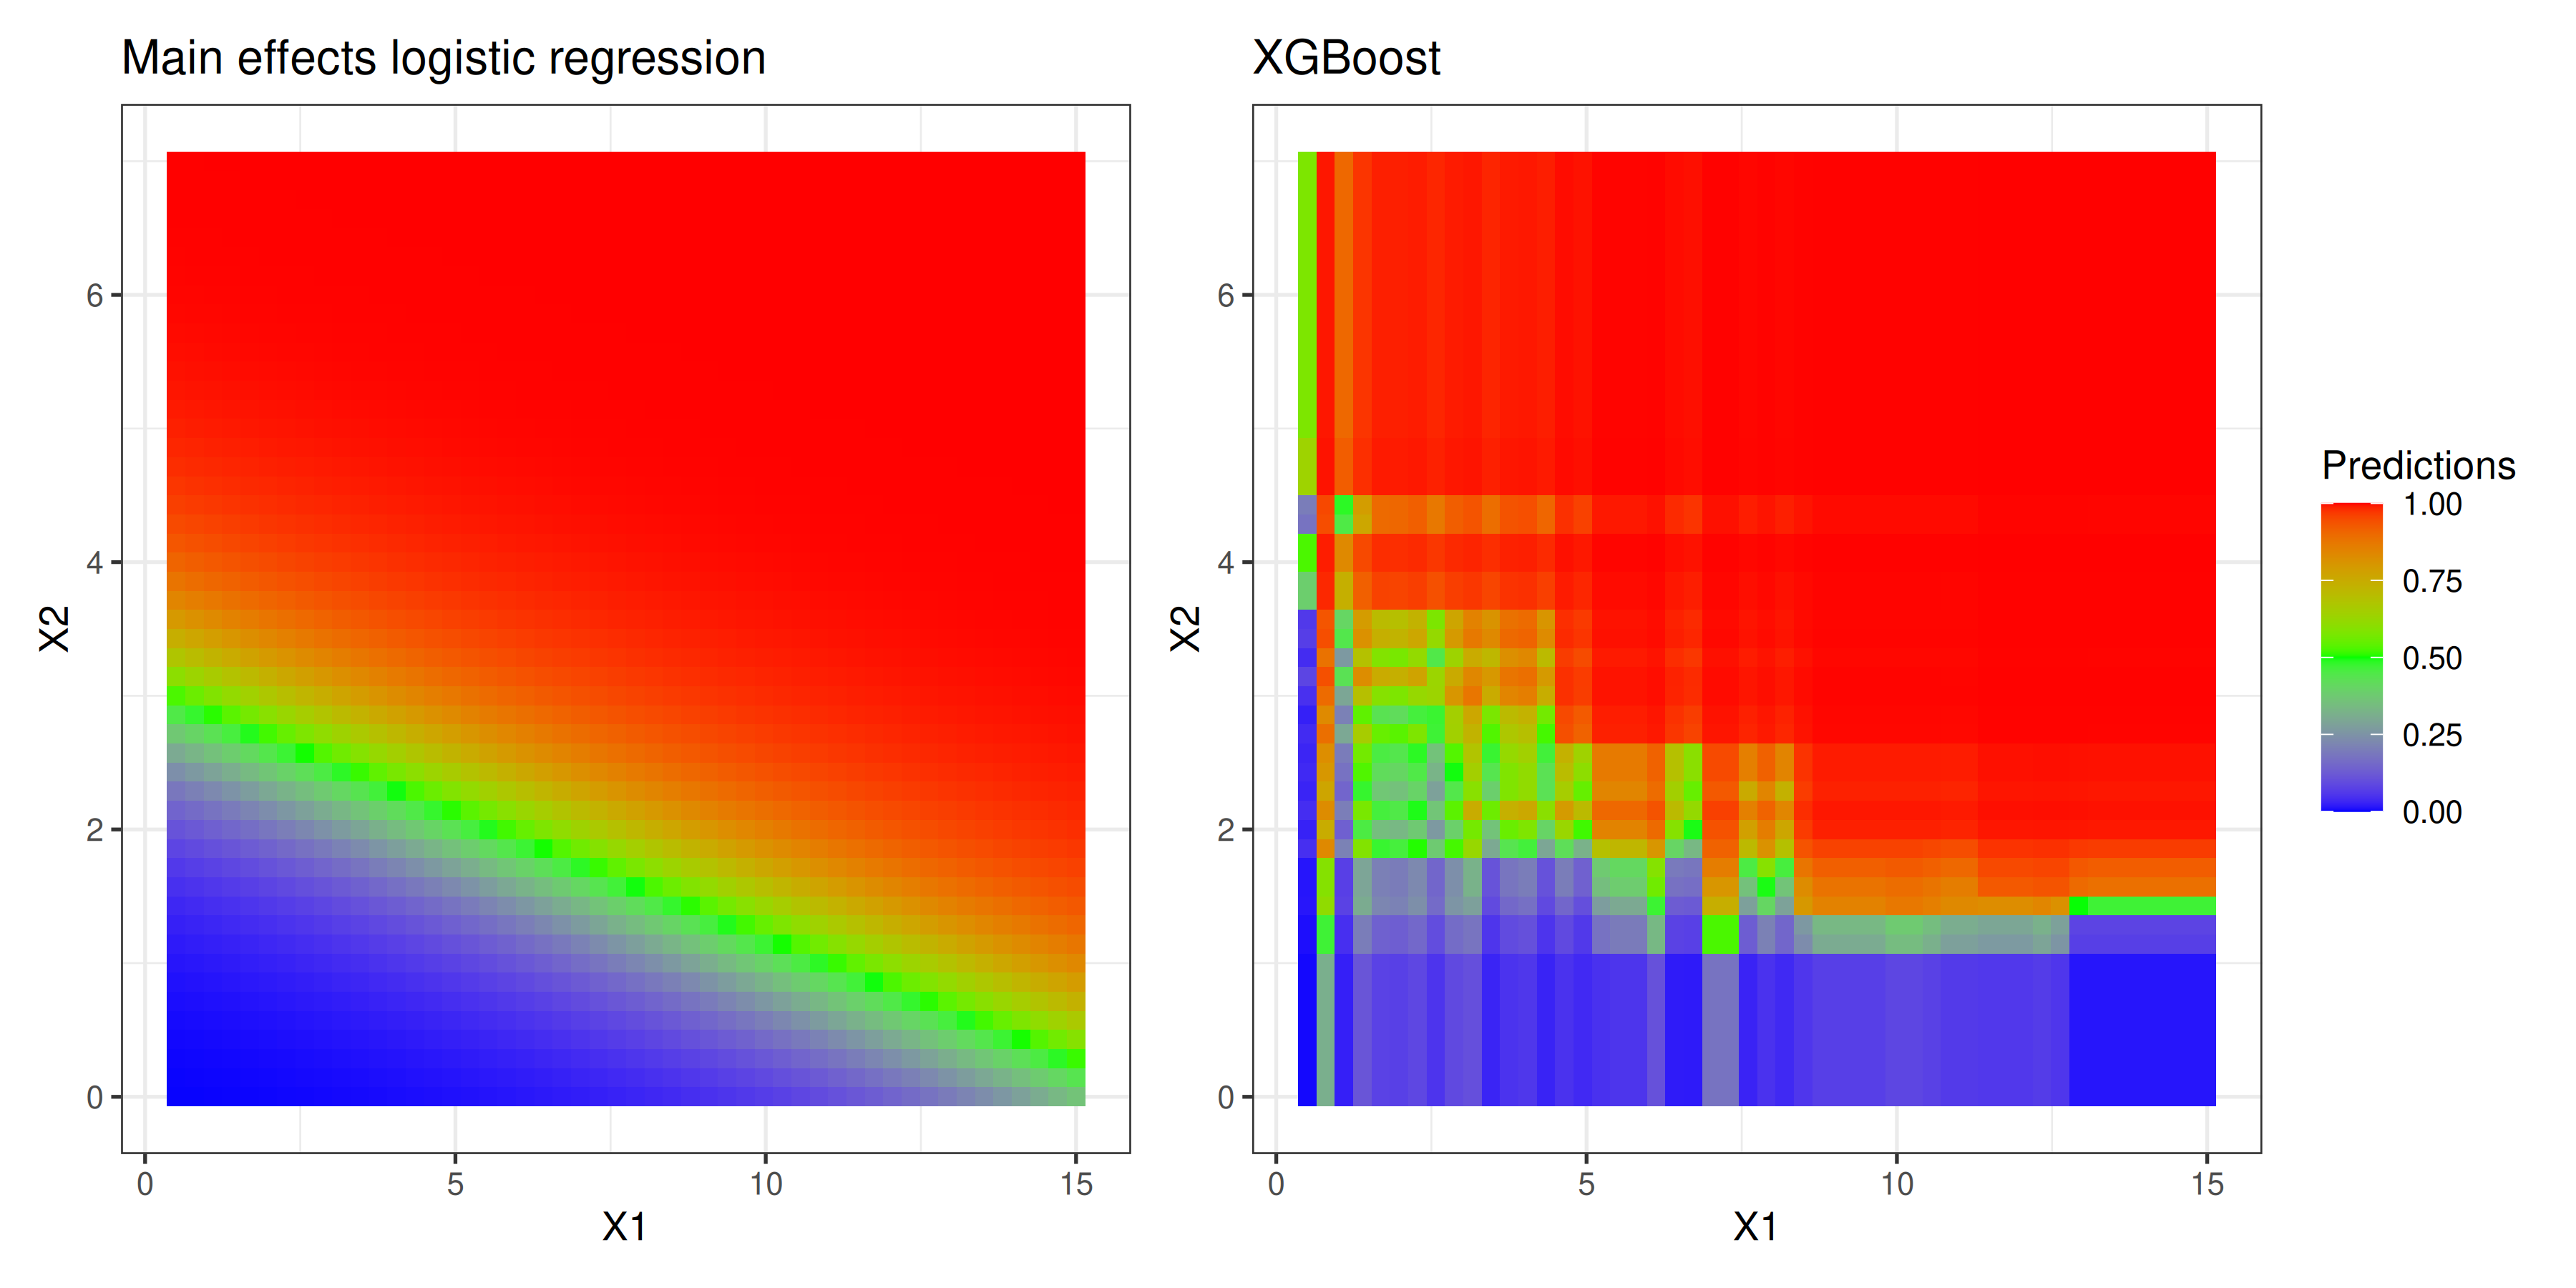
\includegraphics[width=\textwidth]{figures/predictpar.png}
    \caption{The predictions of the main effects logistic regression and XGBoost fitted on 1000 observations}
    \label{fig:predictpar}
\end{figure}

The plot for the intercept only logistic regression is omitted, as its appearance is as one would expect -- the plot is simply an orange square. The intercept only logistic regression is included as a baseline, the predicted probability of the intercept model is simply the average of the observed $ Y_i$'s. 

From figure \ref{fig:predictpar} we can observe a clear difference in the predicted probabilities between the logistic regression and the tree-based XGBoost. The main effects logistic regression is a parametric model that assumes that the regression function is a smooth transformation of the linear predictor $ X\beta $. XGBoost, in contrast, is made up of many decision trees, which explains the patchwork pattern in its prediction plot. For small samples and as we will see in the simulations, XGBoost has a high risk in comparison to the misspecified main effects logistic regression. However, XGBoost becomes increasingly better at approximating the true regression when the number of observations becomes large as seen in figure \ref{fig:xgboost10k}. By applying a super learning algorithm to the library, we will see that the cross-validation selector is able to qualitatively assess and select the best learning algorithm to apply given the amount of data at hand. The cross-validation selector selects the main effects logistic regression in the beginning with few training samples, but as the predictions of XGBoost become more stable with more samples, the selector is likely to shift its preference towards XGBoost.  
\begin{figure}[H]
    \centering
    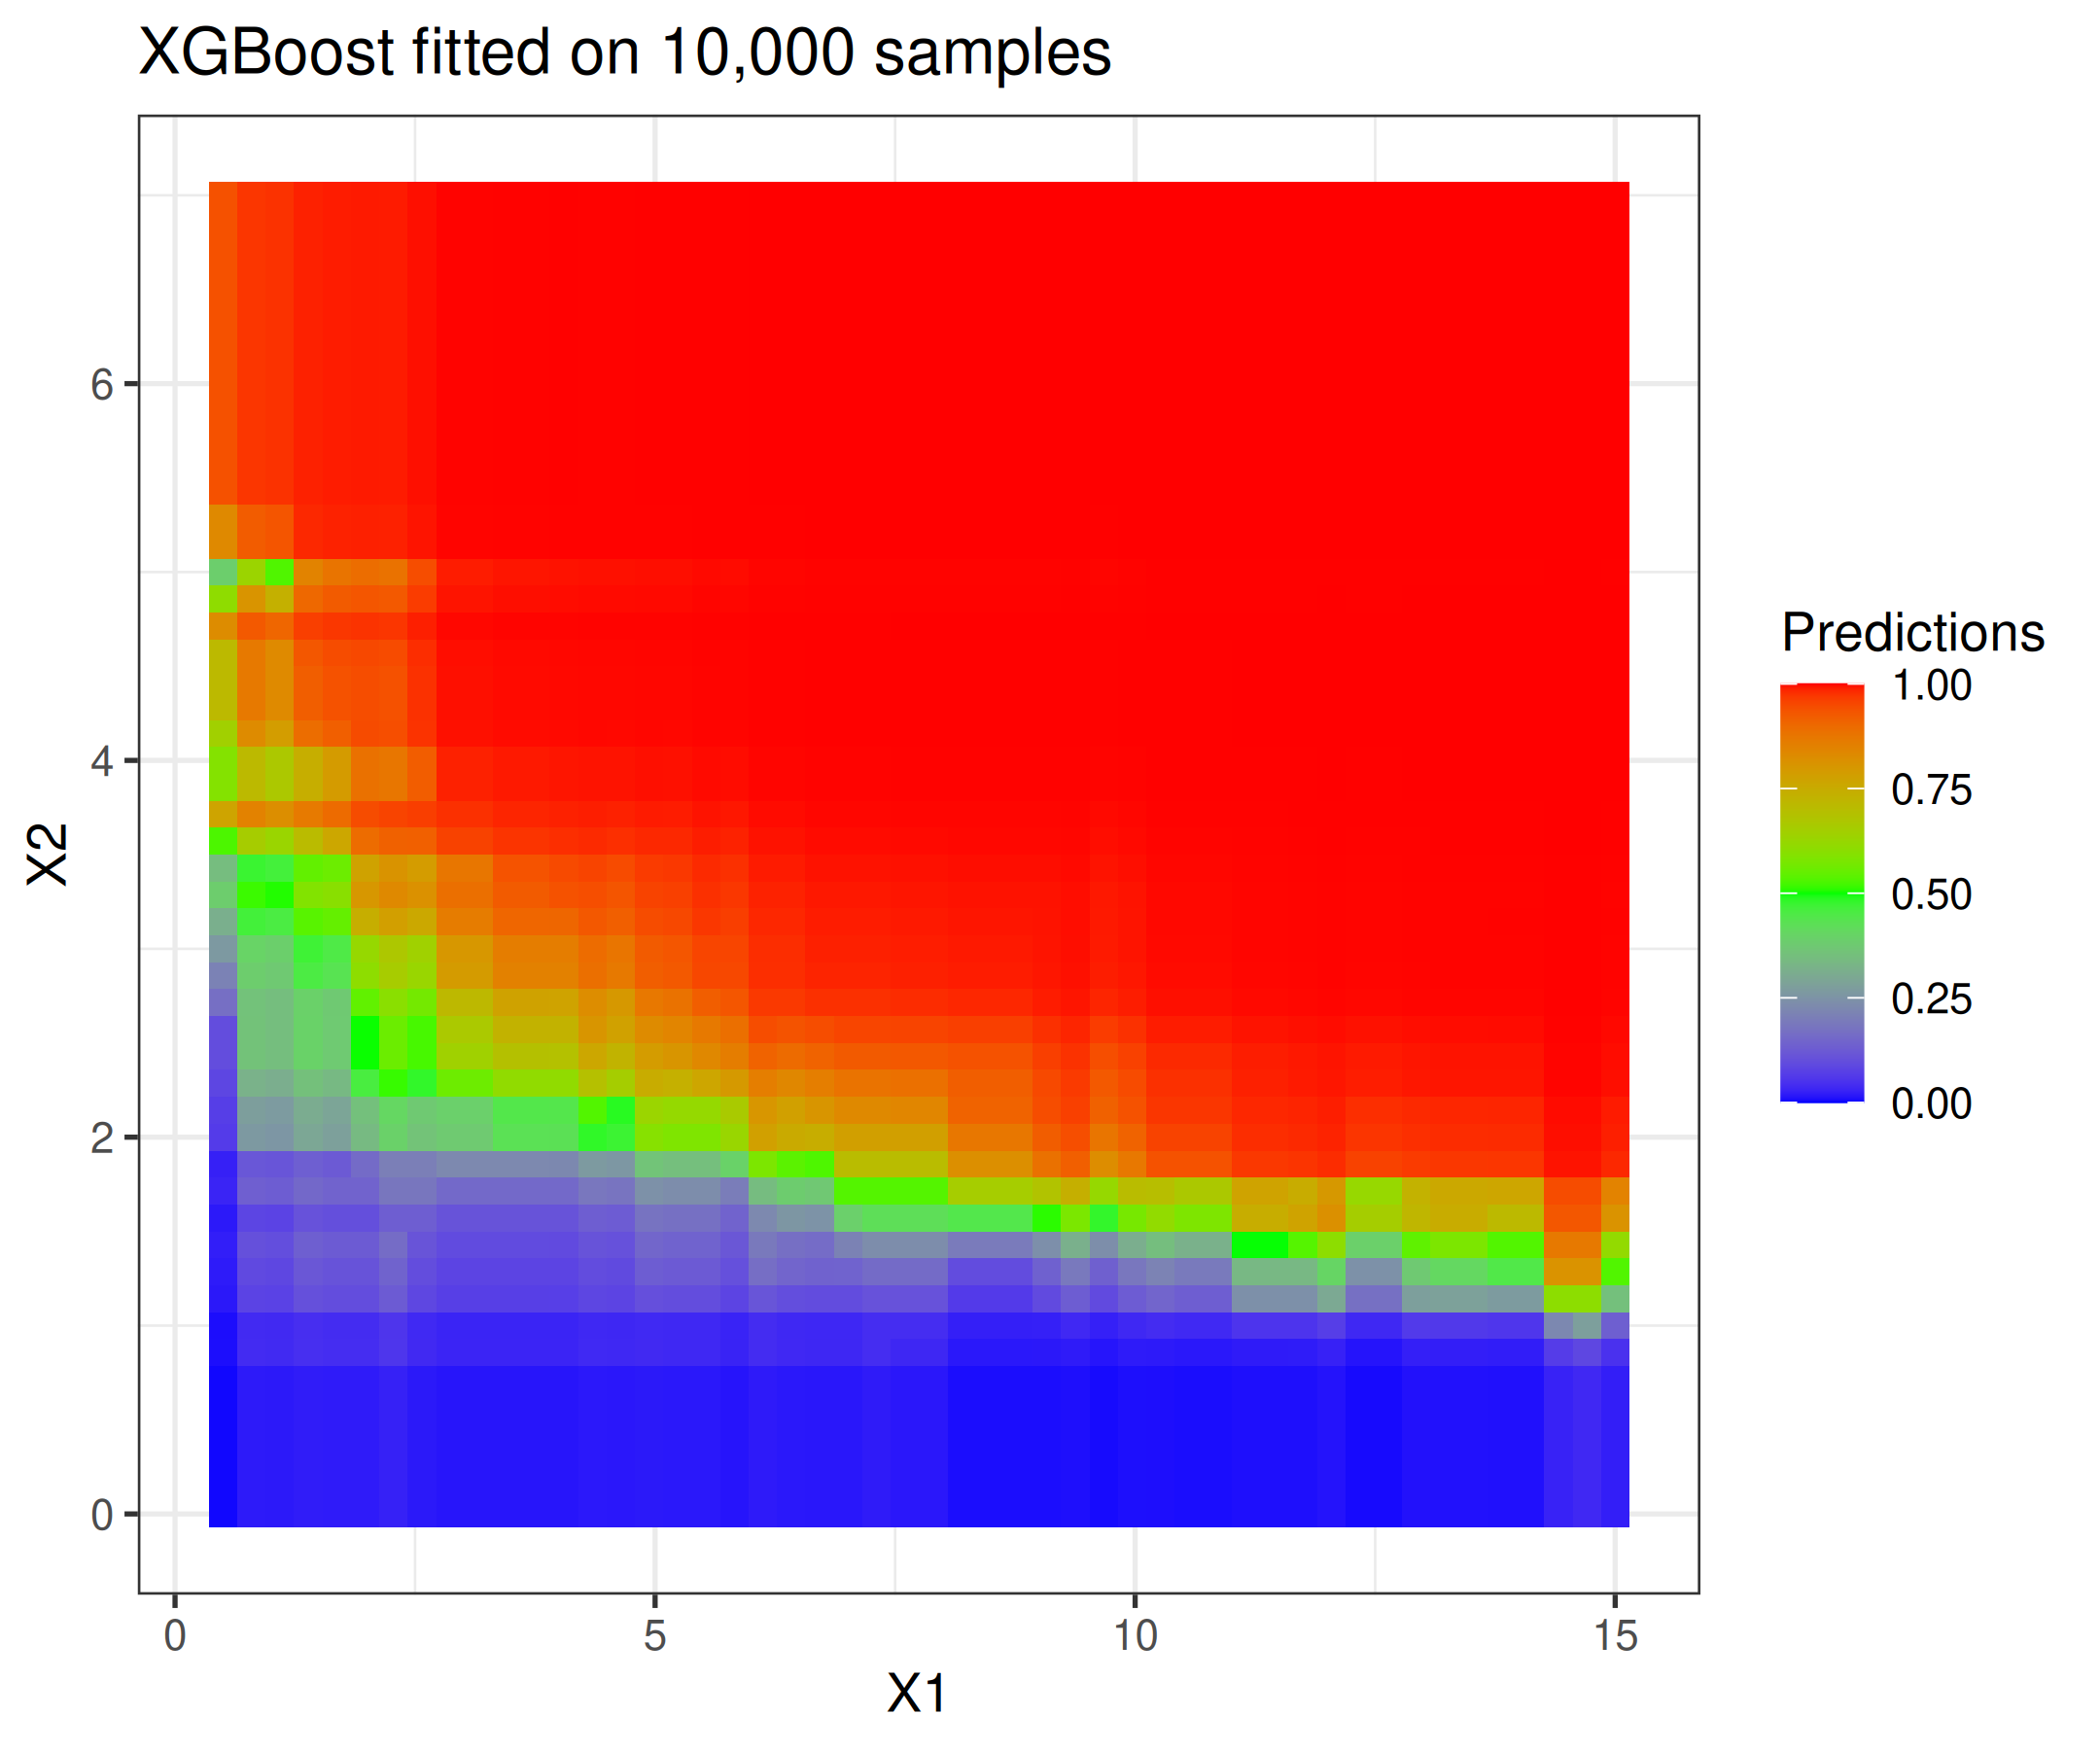
\includegraphics[width=0.7\textwidth]{figures/xgboost10k.png}
    \caption{XGBoost becoming better at approximating the true regression as the sample size increases}
    \label{fig:xgboost10k}
\end{figure}
In our setup, we will consider a discrete super learner that uses 10-fold cross validation and the internal loss function will be the quadratic loss. The performance of the discrete super learner will be compared to each individual learner in the library. We show that
\begin{enumerate}
    \item As the sample size increases, the  discrete super learner achieves the minimum risk 
    \item For a single new observation, the prediction of the discrete super learner on the outcome has the lowest variance
\end{enumerate}
Following is psuedocode for the discrete super learner algorithm:
\begin{algorithm}[H]
\caption{Discrete super learner}
\begin{algorithmic}[1]
\State \textbf{Input:} $D_n$: dataset of size $ n $, $V$: number of folds, $ \lib $: library of learners of size $ k $ 
\State \textbf{Output:} discrete super learner $ \hat{\la}_n(D_n) $
\State \textbf{Initialize:} 
\State $s \gets \text{create folds}(V) $ 
\State $\ell \gets \text{empty matrix of dimensions } V \times k $ // loss matrix 

\For{$s \in \{1, \dots, V\}$}
    \State $D_{n, s}^{1} \gets \{O_i \in D_n \mid s(i) = s\} $
    \State $D_{n, s}^{0} \gets D_n \setminus D_{n,s}^{1} $
    \For{$\la \in \lib$}
    \State $ \la(D_{n,s}^{0}) \gets \text{fit}(\la, D_{n, s}^{0})$
    \State $\ell[s,\la] \gets R(\la(D_{n, s}^{0}), D_{n,s}^{1}) = \frac{V}{n} \sum_{O_i \in D_{n,s}^{1}} L(O_i, \la(D_{n, s}^{0})) $
    \EndFor
\EndFor
\State $ \ell_{\text{final}}(\la) \gets \frac{1}{V} \sum_{s = 1}^{V} \ell[s,\la] $ 
\State $ \hat{\la}_n \gets \argmin_{\la \in \lib} \ell_{\text{final}}(\la) $
\State \textbf{return} $ \text{fit}(\hat{\la}_n, D_n) $
\end{algorithmic}
\end{algorithm}


\subsection{The discrete super learner}
\begin{figure}[H]
    \centering
    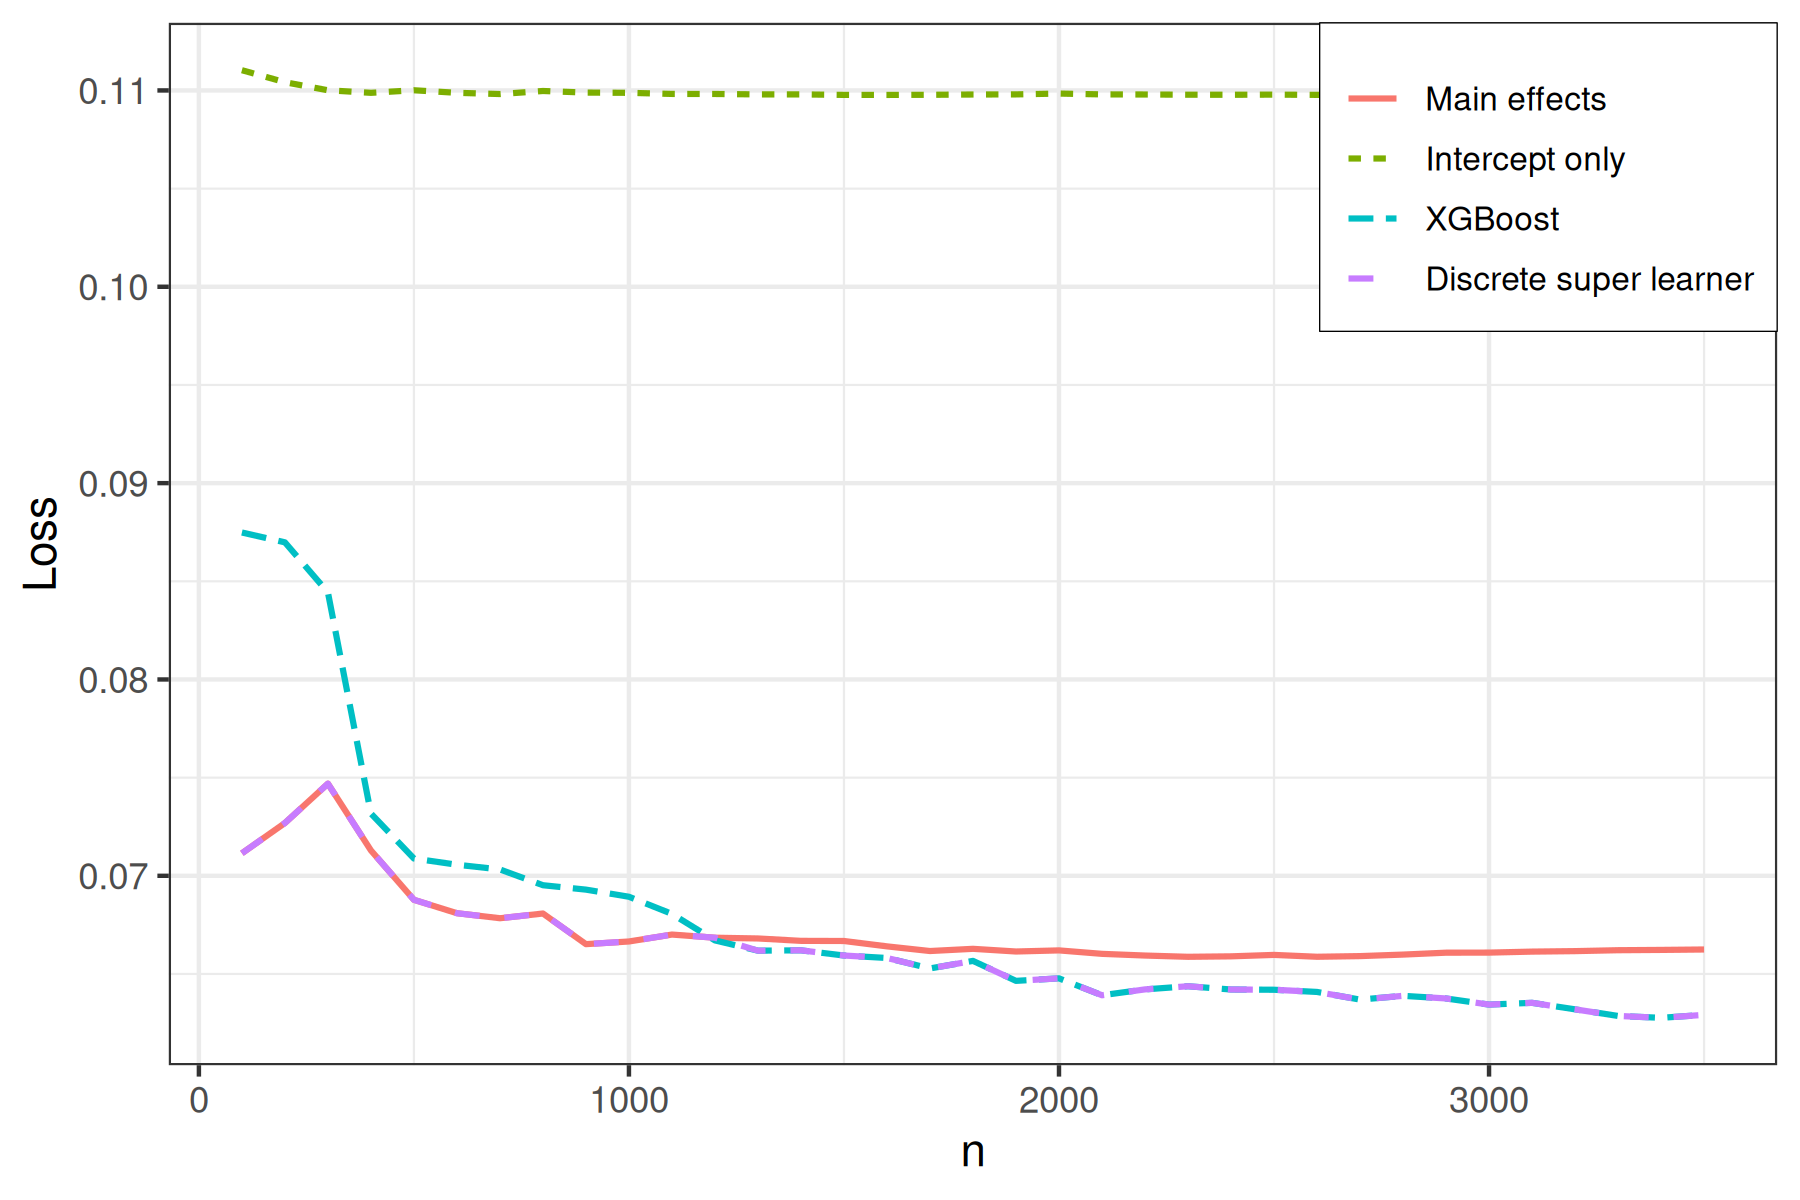
\includegraphics[width=\textwidth]{figures/dsl_loss.png}
    \caption{The risk of the discrete super learner compared to other learners. $ N = 3500 $} 
    \label{fig:loss_min_of_both}
\end{figure}


\begin{figure}[H]
    \centering
    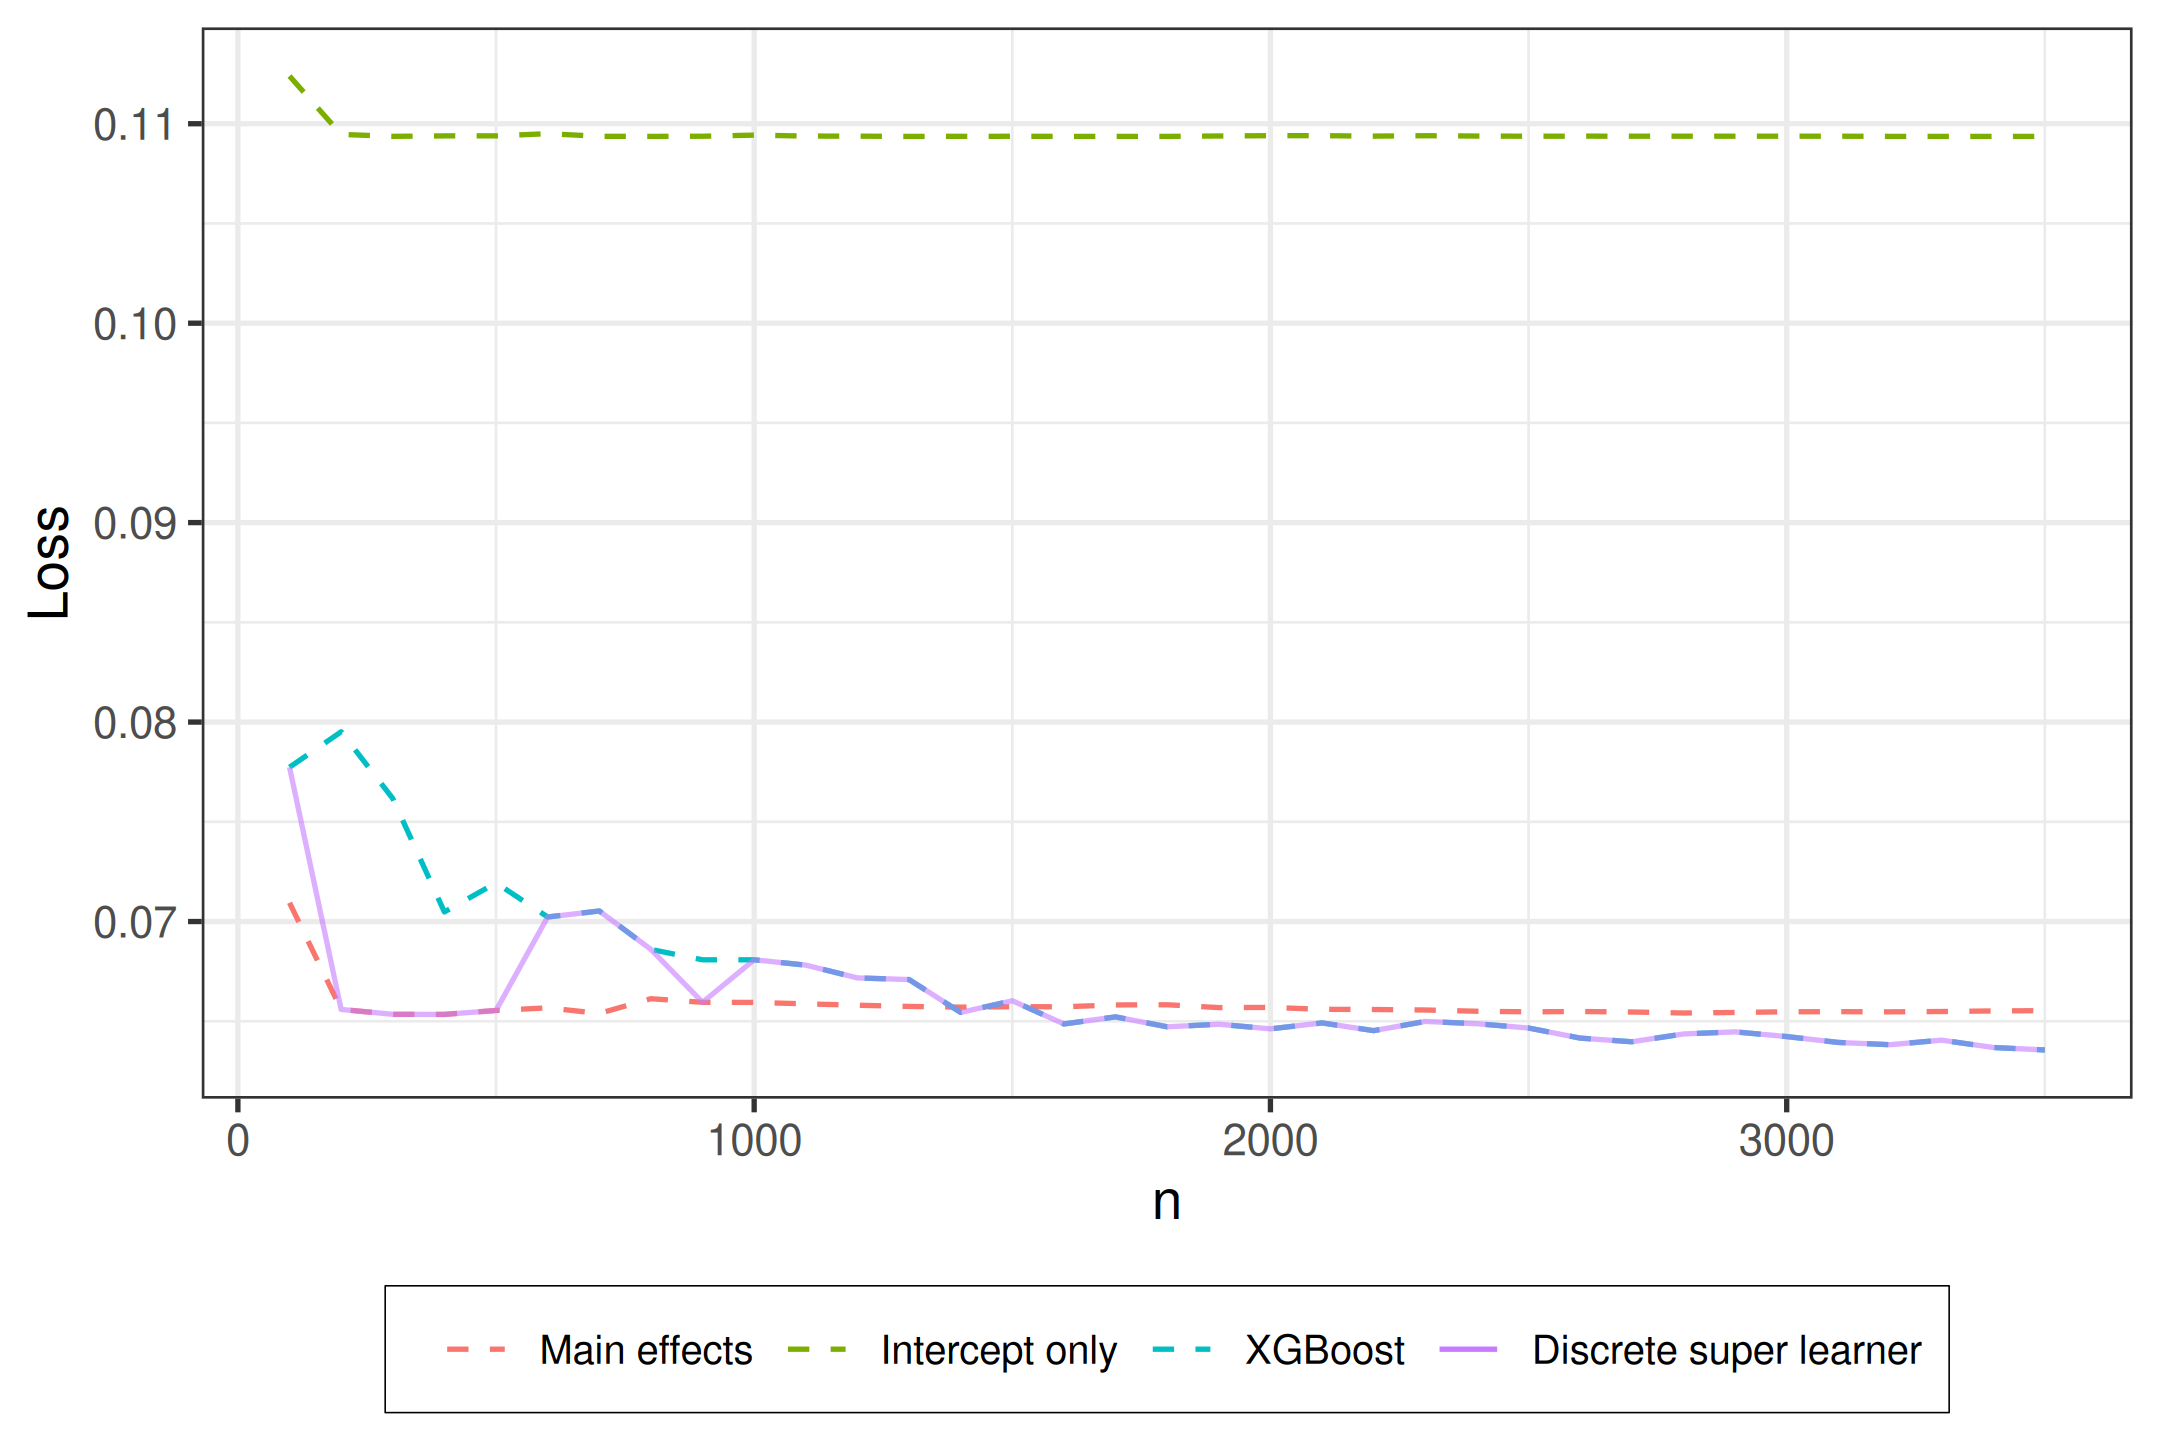
\includegraphics[width=\textwidth]{figures/dsl_loss_jumps.png}
    \caption{The risk of the discrete super learner compared to other learners. $ N = 3500 $}
    \label{fig:loss_jumps}
\end{figure}

\begin{figure}[H]
    \centering
    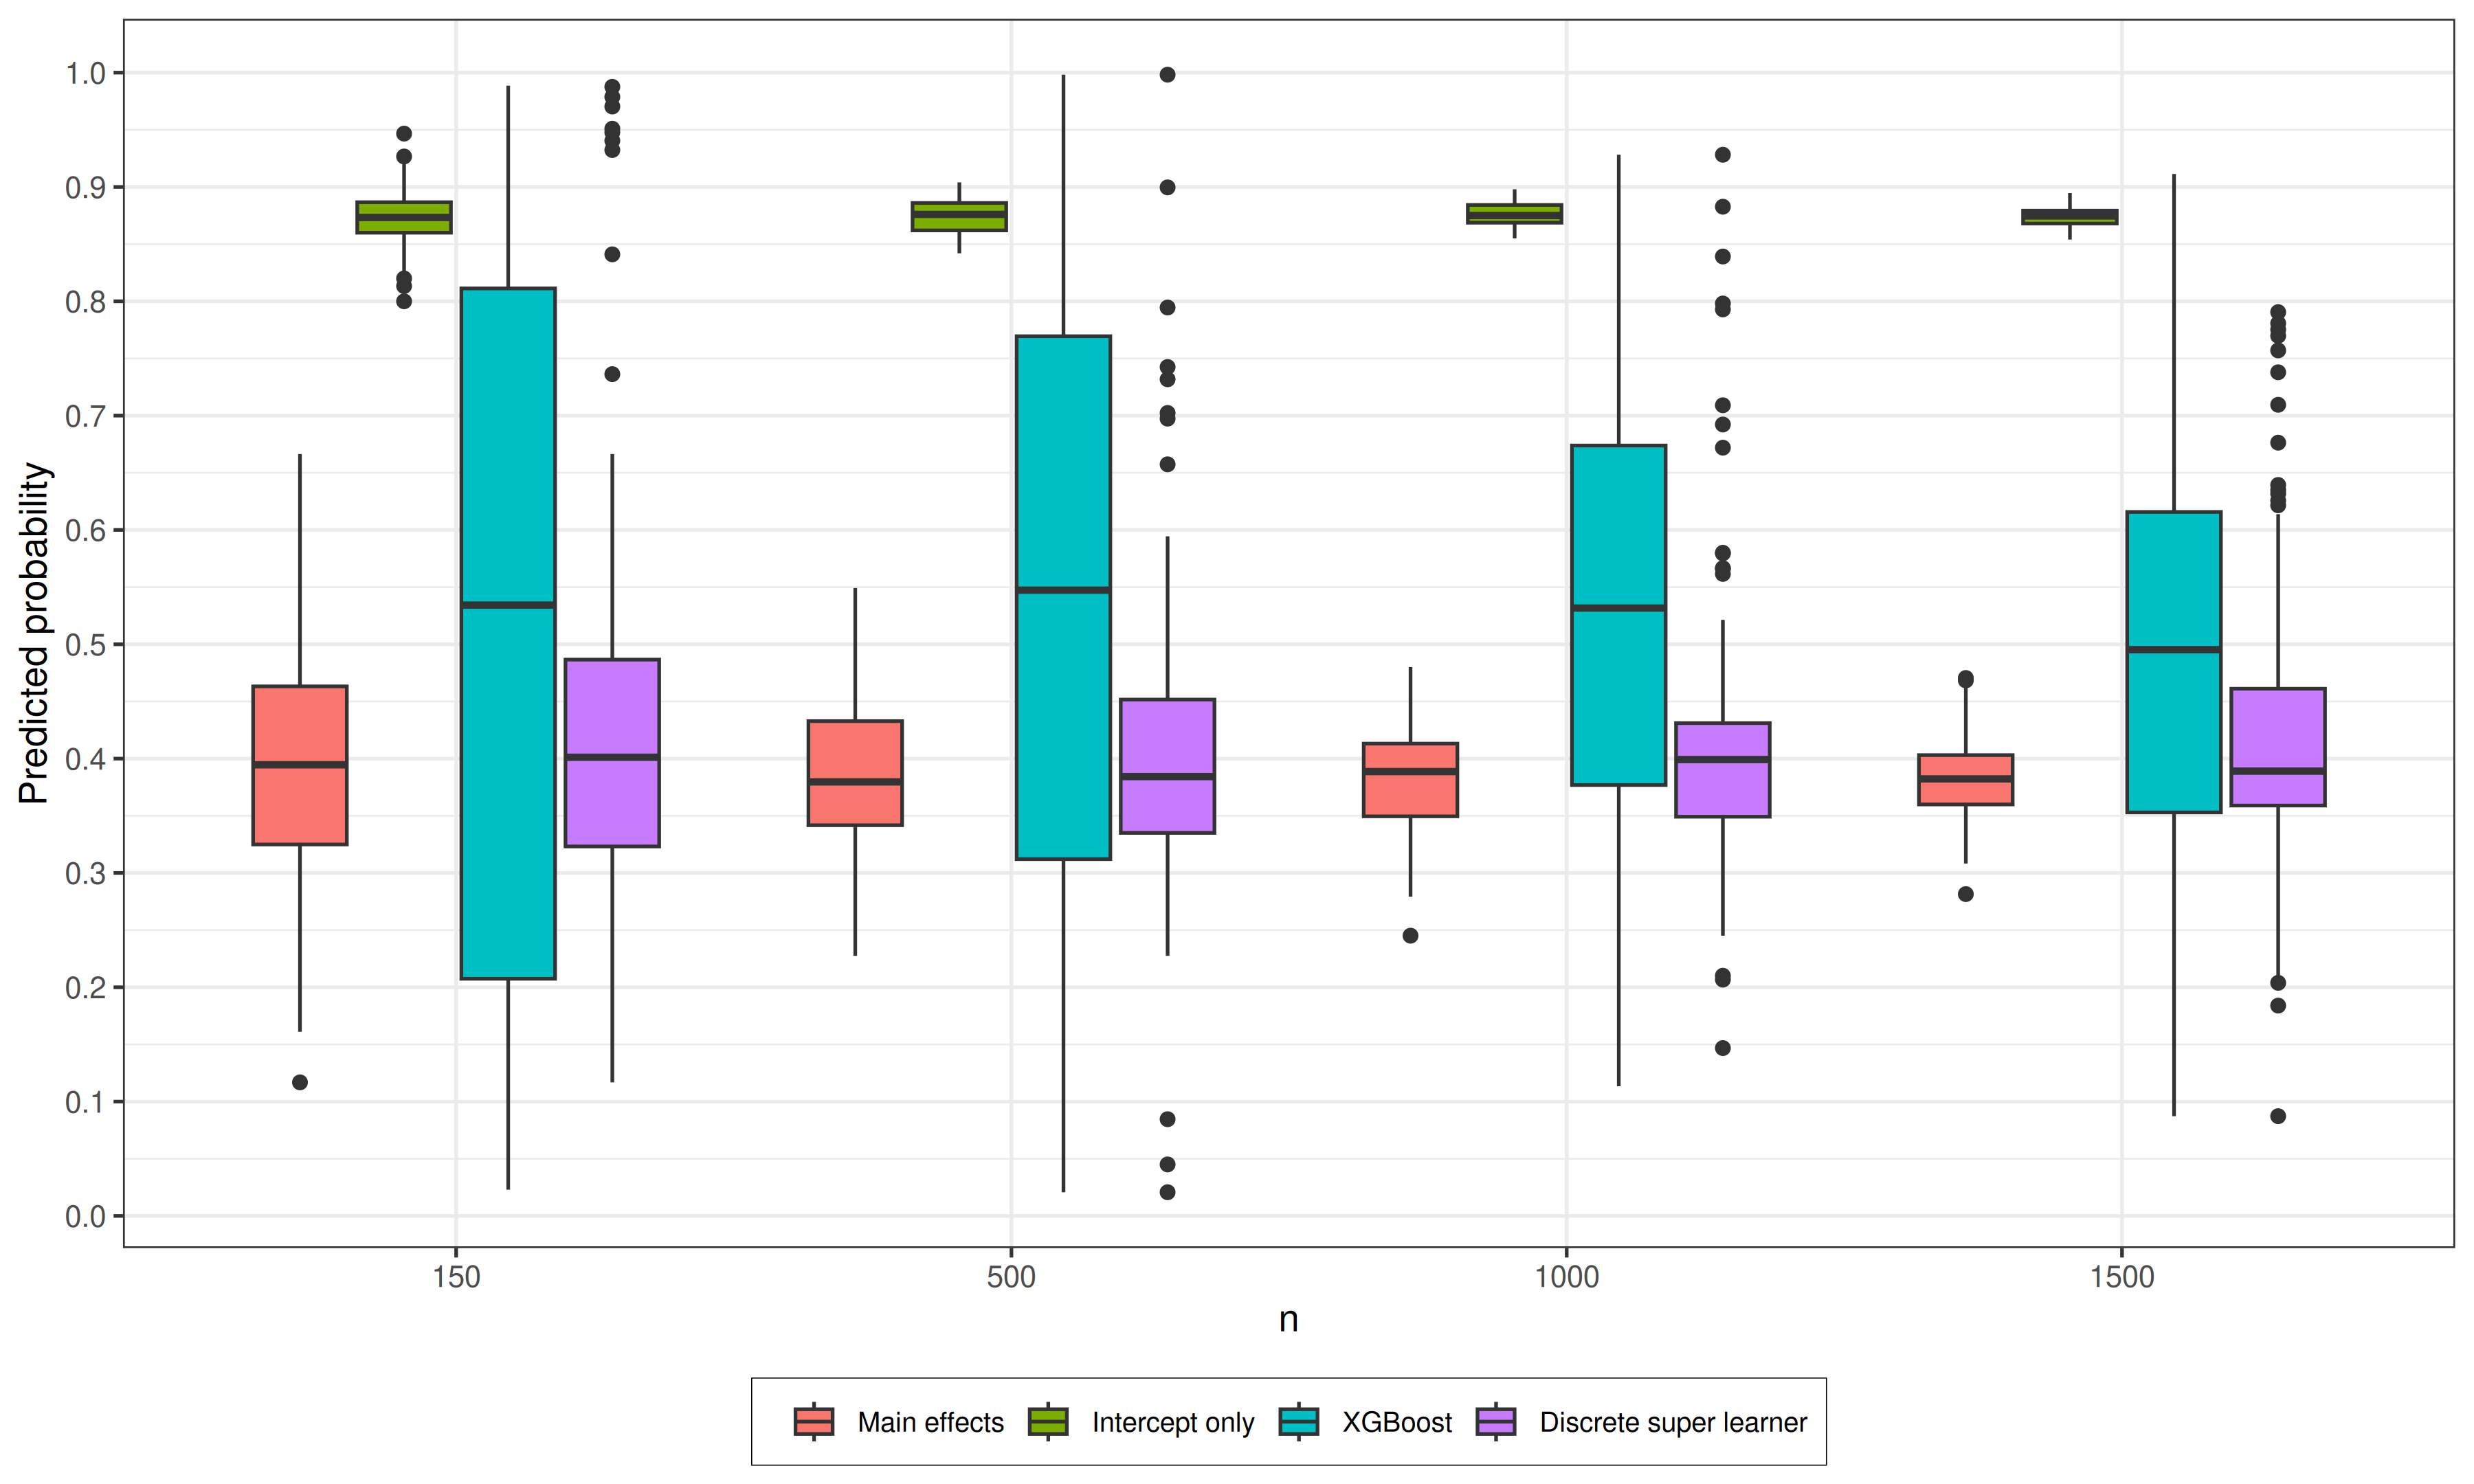
\includegraphics[width=\textwidth]{figures/learner_vars.png}
    \caption{Variances of learner predictions for a single observation, each trained on $n $ samples and evaluated $ K = 1000 $ times on a single observation}
    \label{fig:pred_probs_boxplot}
\end{figure}

\begin{figure}[H]
    \centering
    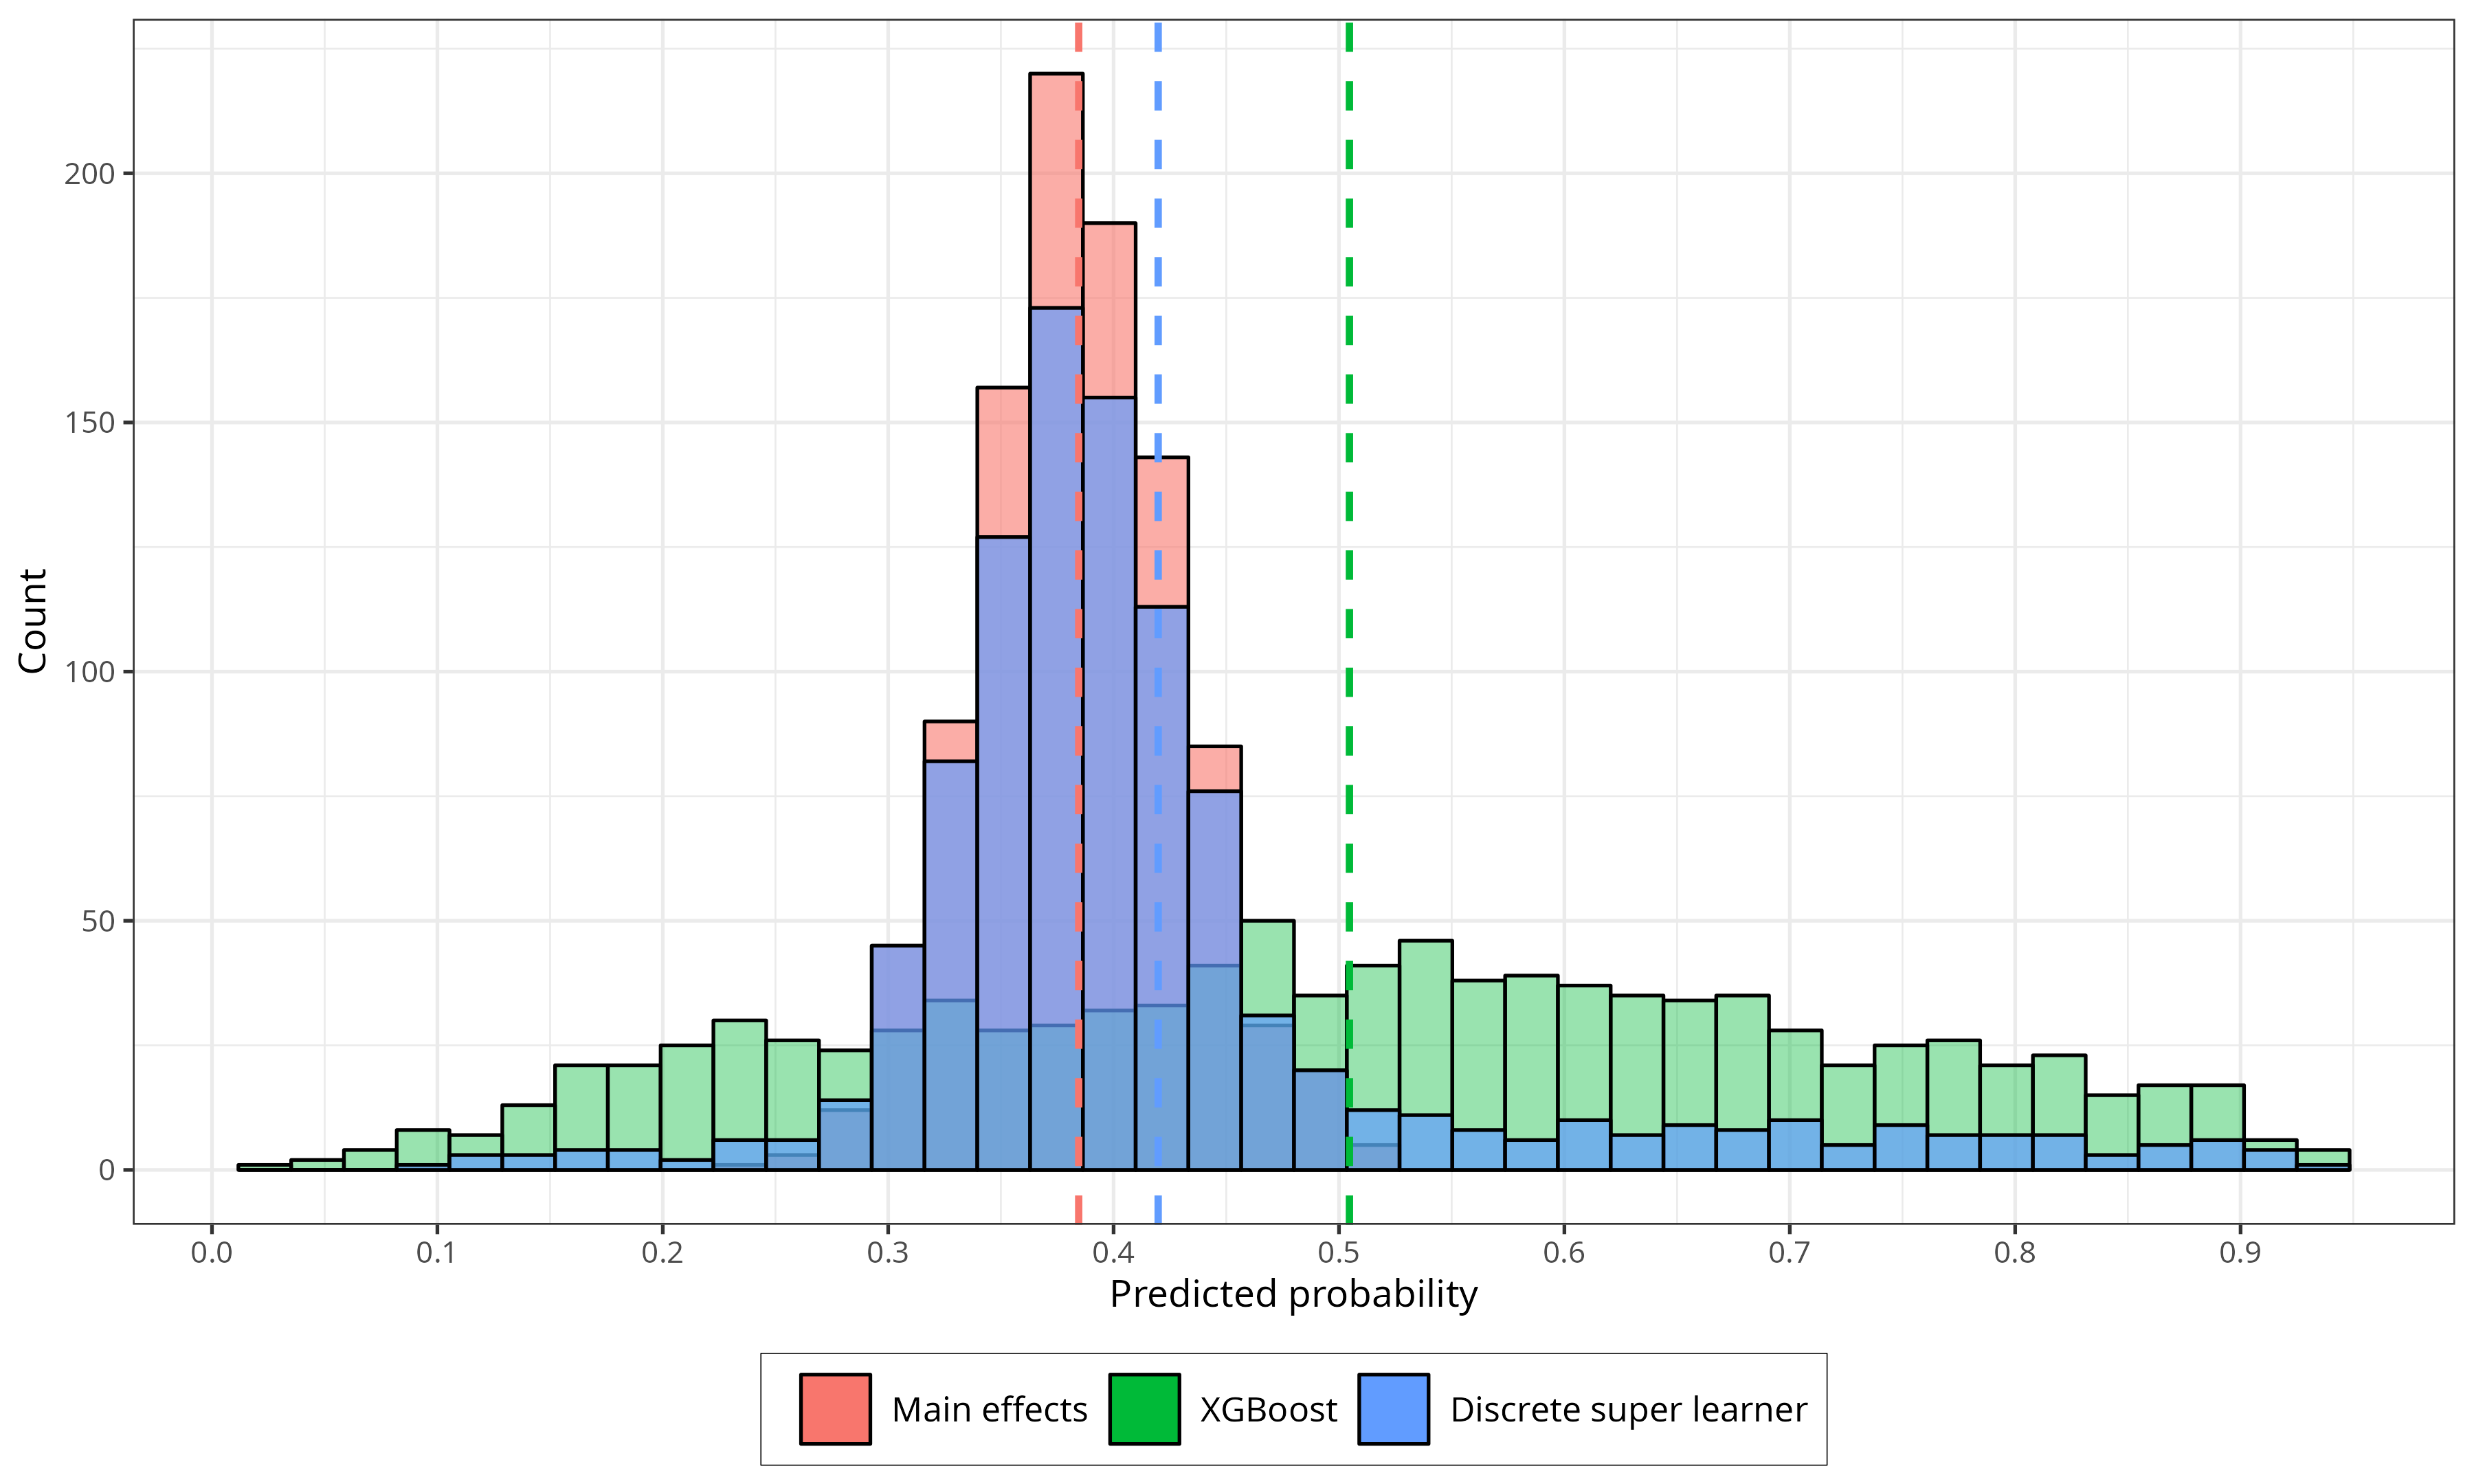
\includegraphics[width=\textwidth]{figures/preds_n1k_dsl.png}
    \caption{Predictions for a single observation by the three learners fitted on $ n = 1000 $}
    \label{fig:dsl_preds_n1k}
\end{figure}

\subsection{Discussion}
Figures \ref{fig:loss_min_of_both} and \ref{fig:loss_jumps} illustrate how the discrete super learner performs in comparison to the learners in terms of loss over number of training samples. The plots are generated for two runs where the model is fitted on $ n = 100, 200, \dots , 3500 $ observations, as indicated on the $ x $-axis, then the empirical risk is calculated by evaluating each fitted learner on a fixed test sample of size of $ 10^{6} $. The test data is sampled from the data-generating distribution.  

The first run perfectly illustrates how the discrete super learner is able to achieve the minimum risk. For small training sample sizes, the machine learning method XGBoost has a higher risk than the main effects logistic regression, and it is therefore more desirable for the discrete super learner to choose logistic regression despite the fact that it is misspecified. The discrete super learner consequently achieves the same risk as the logistic regression in the beginning, but for $ n > 1200 $ the risk of the discrete super learner becomes less than the logistic regression. Here XGBoost begins to achieve a lower risk than the misspecified logistic regression, and so the discrete super learner chooses XGBoost instead. 

The second run shows that the discrete super learner might be unable to determine the learner with the lowest risk when the training sample size is small, which results in it moving in a zig-zag pattern between two learners that have quite similar risks. However, we see that the discrete super learner eventually chooses XGBoost as the training sample size grows.  

Figure \ref{fig:pred_probs_boxplot} illustrates the variance in the predictions of each learner for a single observation, whose true probability is indicated by the red dashed line. Each learner has been trained $ K = 1000 $ times on $ n = 150, 500, \dots 3000 $ samples taken from the distribution and is used to predict $ K $ times after each training. The box plots are created from the $ K $ predictions. 

We observe that the machine learning model, XGBoost, has the highest prediction variance across all training sample sizes. Recall that we only had two covariates, here having 1500 observations limits the range of predictions of our main effects model to be between $ 0.27 $ and $ 0.46 $. Whereas for XGBoost the predictions can vary from below $ 0.1 $ to above $ 0.9 $. While XGBoost is extremely efficient at minimizing loss, its predictions have a high variance unless one has a lot of training data. 

The discrete super learner p
\subsection{The ensemble super learner}
\subsection{Discussion}
\end{document}

